\documentclass[11pt, a4paper]{beamer}
%\usetheme{Berkeley}
%\usetheme{Berlin}
%\usetheme{Copenhagen}
%\usetheme{Antibes}
%\usetheme{Darmstadt} 
\usetheme{Dresden} 

\usecolortheme{sidebartab}
\usepackage[]{movie15}
\usepackage{hyperref}
\hypersetup
{
	colorlinks=true,
	linkcolor=blue,
	filecolor=magenta,
	urlcolor=cyan,
}
\urlstyle{same}

\usepackage{graphicx}
\graphicspath{{./images/}}

\usepackage{movie15}

\begin{document}
	\setbeamertemplate{sidebar left}{}
	\title{Progress Presentation-I}
	\subtitle{e-Yantra Summer Intership-2016 \\ Formation Control of Multiple Swarm Robots}
	
		\author
		{Om Singh\\ Chirag Shah\\
		 \textbf{Mentor 1:} Abhinav Sarkar\\
		 \textbf{Mentor 2:} Avinash Dubey			
		}

	\institute{IIT Bombay}
	
	\date{\today}
	%\addtobeamertemplate{sidebar left}{}{\includegraphics[scale = 0.3]{logowithtext.png}}
	\frame{\titlepage}

\setbeamertemplate{sidebar left}[sidebar theme]
\section{Overview of Project}
\begin{frame}{Overview of Project}

	\textbf{Project Name:} 	 Formation Control of Multiple Swarm Robots\\
	\textbf{Objectives:} \\
		\begin{enumerate}
		
		
			\item Implement formation control over a group of Spark V robot using overhead camera and aruco markers for localization of the robot
			\item Implement swarm behaviors like disperse, follow the leader etc
		\end{enumerate}
	
	\textbf{Deliverables:}
	\begin{itemize}
		\item Robots capable of making any desired formation
		\item Robots capable of implementing Swarm behaviors
	\end{itemize}
	%\\ A group of robot that can form any desired formation as 
	%\\ specified by user.\\ 

\end{frame}

\section{Overview of Task}
\begin{frame}{Overview of Task}

		\begin{tabular}{|c|c|c|}
			\hline
			\textbf{No.} & \textbf{Task} & \textbf{Deadline}\\
			\hline
			1.& Python,Spark V ,OpenCV&2days\\& introduction interface Xbee&   \\
			\hline
			2. & Position and orientation & 3 Days \\&calculation of multiple Spark V robots & \\
			\hline
			3. &  Go-to-goal for a single Spark V & 4 Days\\
			\hline
			4. &  Formation testing for 2-3 robots & 2 Days\\
			\hline
			5. &  Algorithm for formation control of  & 3 Days\\ &multiple robots & \\
			\hline
			6. & Avoid obstacle controller & 3 Days\\
			\hline
			7. & Algorithm testing and fine tuning & 3 Days\\ & Scaling up the number of robots & \\
			\hline
			8. & Local Swarm behaviors & 8 Days\\
			\hline
		\end{tabular}	
\end{frame}

\section{Task Accomplised}
\begin{frame}{Task Accomplished}
	\textbf{Task Completed}
	\begin{itemize}	
	\item Cropping and transforming the arena area inside the black border
	%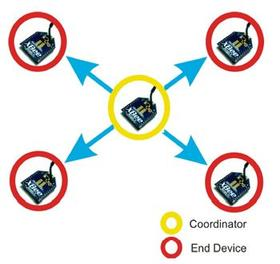
\includegraphics[scale =.2]{2.jpg}
		\item The position and orientation (x, y,$\Phi$) of Multiple robots can be found using aruco markers placed on the robot\\
		
\includegraphics[scale =.1]{images/aruco.jpg}
		
		
		 Opencv-Contrib-python (aruco library)\\ \url{https://github.com/opencv/opencv_contrib}
\end{itemize}
\end{frame}	

\begin{frame}{Task Accomplished}
\begin{itemize}

		\item Selected suitable equations for the differential drive robot\\
		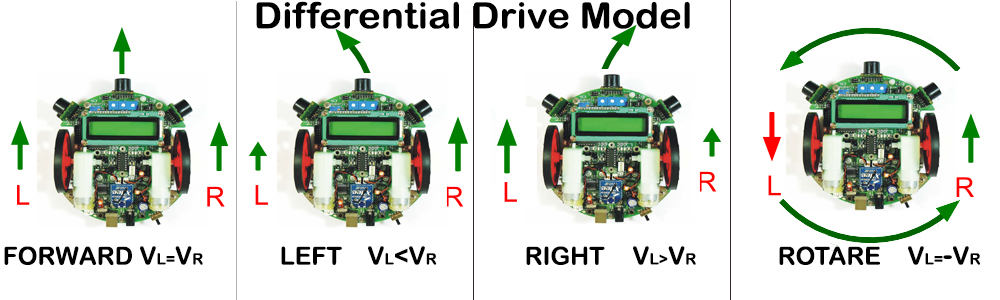
\includegraphics[scale =.4]{images/ddrive.jpg}
		\item (x, y, $\theta$) of each robot is transmitted via XBee to the robot. The desired location (xg,yg,$\phi$) is also transmitted. The XBees are configured in a star configuration
		\\ \begin{center}
			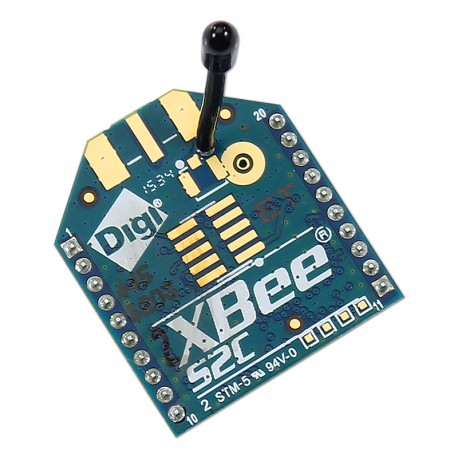
\includegraphics[scale =.12]{images/xbee.jpg}
			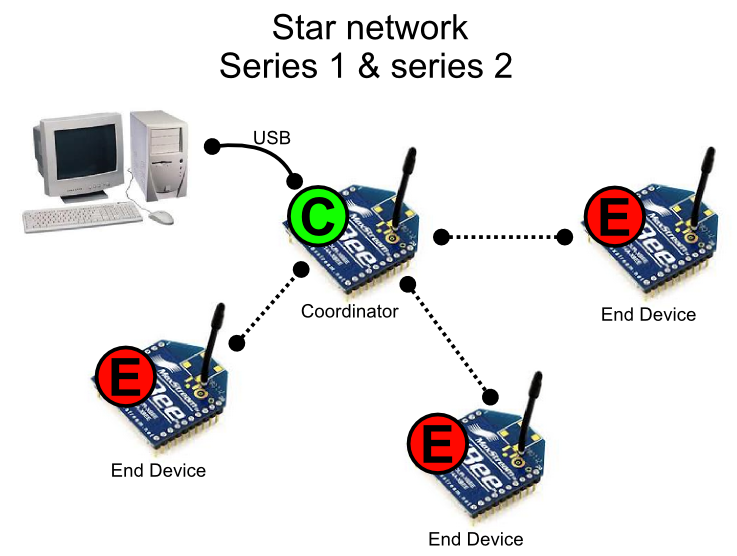
\includegraphics[scale =.12]{images/star.png}
			\end{center}
\end{itemize}
\end{frame}

\begin{frame}{Task Accomplished}

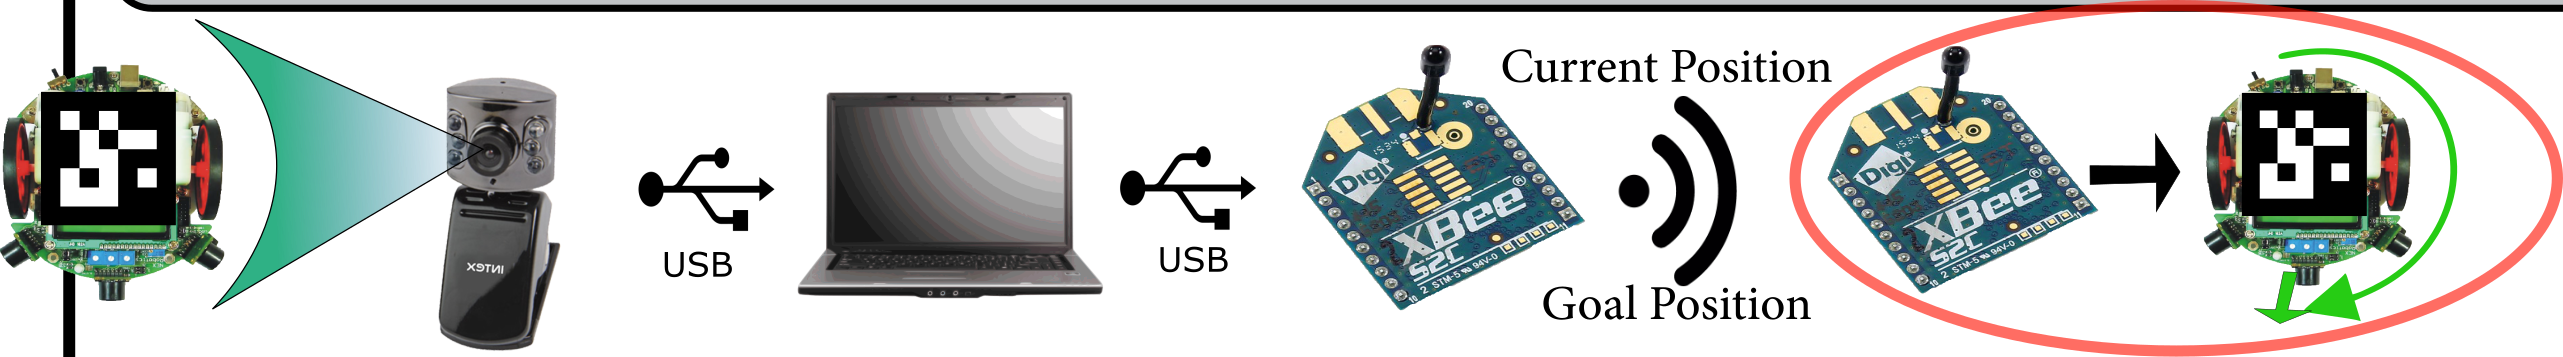
\includegraphics[scale =.4]{images/flow.png}
\begin{itemize}
		\item The robot can turn and move towards the required location using a P controller for differential drive\\	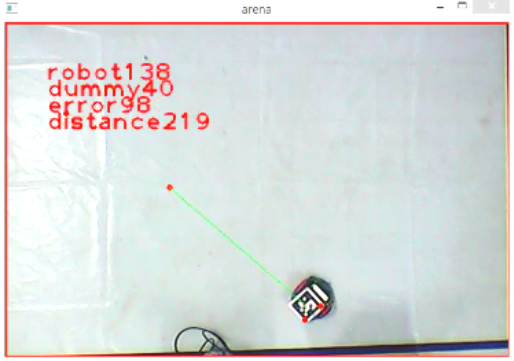
\includegraphics[scale =.35]{images/snip0.png}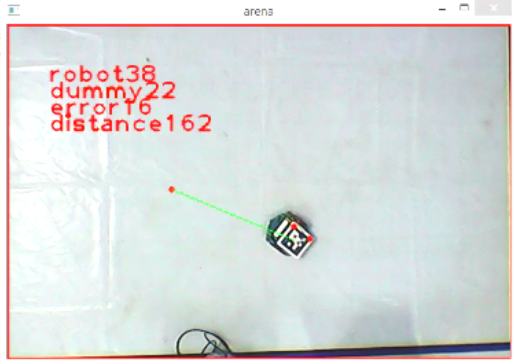
\includegraphics[scale =.35]{images/snip1.png}\\
	\end{itemize}
\end{frame}

%\begin{frame}{Task Accomplished}
%	\begin{figure}[ht]
%		\includemovie[]{2cm}{2cm}{1.avi}
%	\end{figure}
%\end{frame}

\section{Next Tasks}
\begin{frame}{Next Tasks}
\begin{itemize}
	\item Implementing a PID controller on the robot to increase the precision of Go-To-Goal	
	\item Go-to-Goal for multiple robots
	
\end{itemize}	
\end{frame}

\section{Challenges Faced}
\begin{frame}{Challenges Faced}
	\begin{itemize}
%		\item Aruco detection on Open cv.
		\item Communication between computer(Master) and robot(Slave) to transmit the robots initial state and desired state\\ (x, y, $\Phi$)(Serial Communication Protocol)
		\item Developing an effective differential drive robot  model for the Spark V
		\item Conversion from unicycle model to differential drive model
		\item Implementing  Go-to-goal controller using P controller algorithm on the Spark V
	\end{itemize}
\end{frame}

\section{Future Plans}
\begin{frame}{Future Plans}
	\begin{itemize}
	\item Communication of Master(PC) to Multiple slaves(Spark V)
		\item Multiple robots capable of moving to a point selected manually
		\item Multiple robots making pre-defined formation
		\item Swarm behaviors like "follow the leader"
	\end{itemize}
\end{frame}


\section{Thank You}
\begin{frame}{Thank You}
	\centering \textbf{THANK YOU !!!}
\end{frame}
\end{document}
